\section{WebGL}

\subsection{Pipeline}
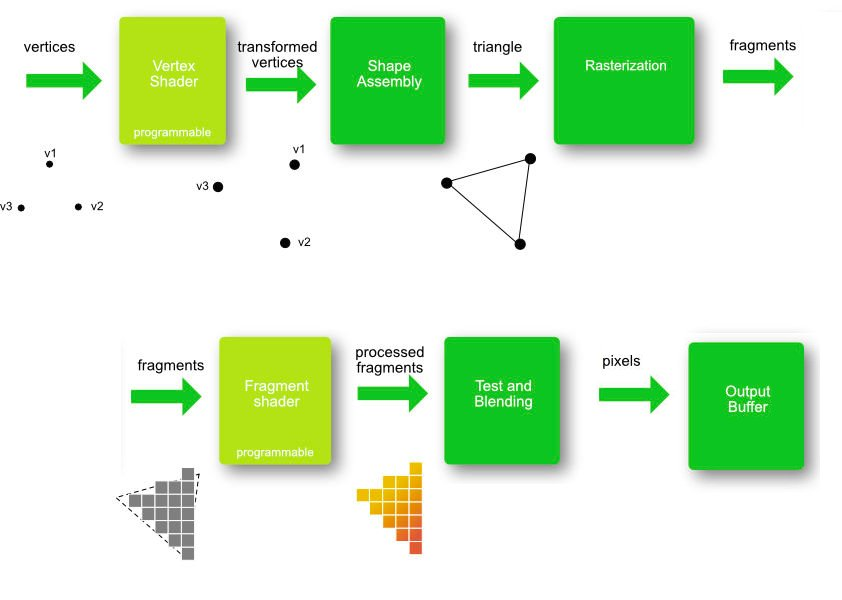
\includegraphics[width=0.9\textwidth]{images/graphicPipeline.jpg}

\subsection{Buffers: webGL's abstract data-structures}

First, we need to explain some jargon. 
\begin{itemize}
    \item \emph{context}: a set of slots that users can access to manipulate data. Most important slot: \inlinecode{gl.ARRAY_BUFFER}
    \item \emph{buffer}: a object of data that can be provided to a shader.
\end{itemize}

Passing data in to webGL: 
\begin{itemize}
    \item Generate a buffer and get its id: \inlinecode{let id: number = gl.createBuffer();}
    \item The \inlinecode{ARRAY_BUFFER} is a place where a buffers data may be modified. \inlinecode{gl.bindBuffer(gl.ARRAY_BUFFER, id);}
    \item Put in actual data. \inlinecode{gl.bufferData(gl.ARRAY_BUFFER, [1.2, 3.2, 4.0], gl.STATIC_DRAW);}
\end{itemize}


\subsection{Shaders}

\subsubsection{Shader basics}

\paragraph{The vertrex shader} is called once for every vertex. It does some transformation on the vertex to add perspective and then stores the result in \inlinecode{gl_Position}. 
Note that these shaders cannot add vertices, they can only modify them. A good usage example is motion-distortion (making objects passing by look distorted) or water rippeling.

\paragraph{The fragment shader} is called once for every pixel on every shape. It determines the pixel's color (\inlinecode{gl_FragColor}) by
\begin{itemize}
    \item which pixel of a texture belongs here, 
    \item applying lighting and shadows
\end{itemize} 

\subsubsection{Attributes and uniforms}

\paragraph{attributes} In WebGL, values that apply to a specific vertex are stored in attributes. These are only available to the JavaScript code and the vertex shader. Attributes are referenced by an index number into the list of attributes maintained by the GPU. 
Since attributes cannot be used unless enabled, and are disabled by default, you need to call \inlinecode{enableVertexAttribArray()} to enable individual attributes so that they can be used. Once that's been done, other methods can be used to access the attribute, including \inlinecode{vertexAttribPointer(), vertexAttrib*()}, and \inlinecode{getVertexAttrib()}.


Once the data is in the buffer we need to tell WebGL how to get data out of it and provide it to the vertex shader's attributes.

To do this, first we ask WebGL what locations it assigned to the attributes. For example in the code above we have
\begin{lstlisting}[language=c]
    // look up where the vertex data needs to go.
    var positionLocation = gl.getAttribLocation(program, "a_position");
    var colorLocation = gl.getAttribLocation(program, "a_color");
\end{lstlisting}
This is also usually done at initialization time.

Once we know the location of the attribute we then issue 3 commands just before drawing.
\begin{lstlisting}[language=c]
    // That command tells WebGL we want to supply data from a buffer.
    gl.enableVertexAttribArray(location);

    // That command binds a buffer to the ARRAY_BUFFER bind point. 
    // It's a global variable internal to WebGL
    gl.bindBuffer(gl.ARRAY_BUFFER, someBuffer);


    //  And that command tells WebGL to get data from the buffer that is 
    // currently bound to the ARRAY_BUFFER bind point, how many components per vertex (1 - 4), 
    // what the type of data is (BYTE, FLOAT, INT, UNSIGNED_SHORT, etc...), 
    // the stride which means how many bytes to skip to get from one piece of data 
    // to the next piece of data, and an offset for how far into the buffer our data is.
    gl.vertexAttribPointer(
        location,
        numComponents,
        typeOfData,
        normalizeFlag,
        strideToNextPieceOfData,
        offsetIntoBuffer);
\end{lstlisting}

Number of components is always 1 to 4. If you are using 1 buffer per type of data then both stride and offset can always be 0. 0 for stride means "use a stride that matches the type and size". 0 for offset means start at the beginning of the buffer. Setting them to values other than 0 is more complicated and though it has some benefits in terms of performance it's not worth the complication unless you are trying to push WebGL to its absolute limits.
